\begin{figure*}[t]\centering
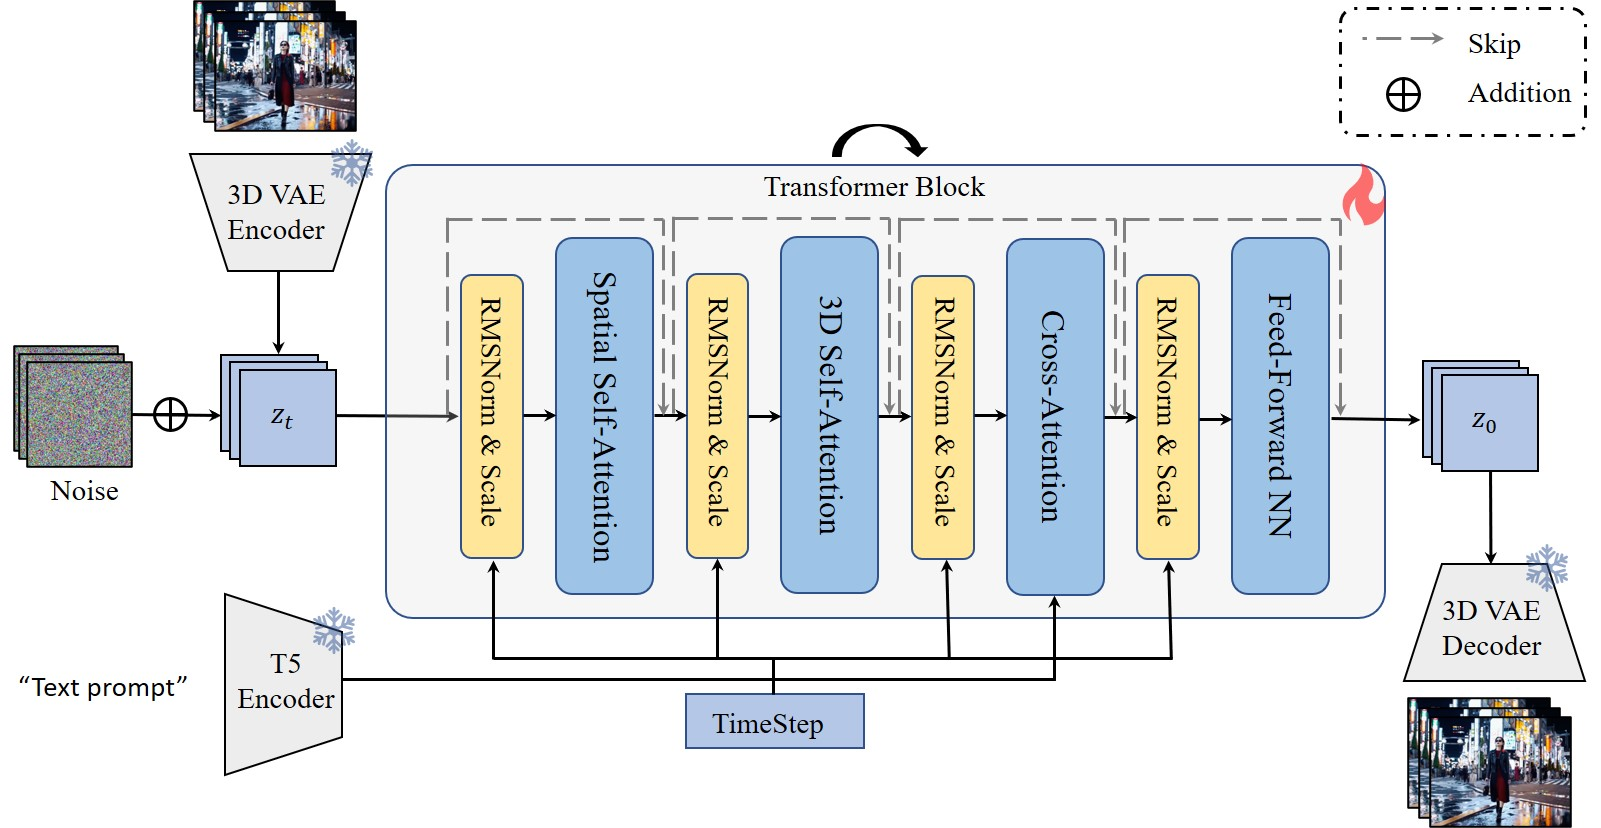
\includegraphics[width=0.6\textwidth]{figures/fig_basemodel.jpg}
\caption{\text{Overview of the base text-to-video generation model.}}
    \label{fig_basemodel}
\end{figure*}
% \input{fig_tab_texs/fig_dataset}
\section{Introduction of the Base Text-to-Video Generation Model}
We use a transformer-based latent diffusion model as the base T2V generation model, as illustrated in Fig. \ref{fig_basemodel}. We employ a 3D-VAE to transform videos from the pixel space to a latent space, upon which we construct a transformer-based video diffusion model. Unlike previous models that rely on UNets or transformers, which typically incorporate an additional 1D temporal attention module for video generation, such spatially-temporally separated designs do not yield optimal results. We replace the 1D temporal attention with 3D self-attention, enabling the model to effectively perceive and process spatiotemporal tokens, thereby achieving a high-quality and coherent video generation model. Specifically, before each attention or feed-forward network (FFN) module, we map the timestep to a scale, thereby applying RMSNorm to the spatiotemporal tokens.
\section{Details of Collected Dataset}
% To implement our method, we require large-scale multi-scene long videos with precise camera annotations. We collected such data using Unreal Engine 5. Fig.~\ref{fig:dataset} showcases our $12$ diverse scenes, including large-scale environments like factories, islands, and cities. We collected $100$ long videos across these scenes, with each sequence containing $7601$ frames. The camera parameters in Unreal Engine 5 were set to $24.0$ mm focal length and $10.0$ aperture. For camera trajectories, we constrained position changes to the x and y axes, and rotation changes to yaw (z-axis rotation) only. Starting from random points in scenes, we generated continuous trajectories between randomly selected endpoints while avoiding model penetration. The distance between consecutive endpoints was no more than $600$ cm, with rotation changes not exceeding $60$ degrees. Each segment between consecutive endpoints spans $77$ frames.

In this section, we provide a detailed description of the rendered dataset used to train our model.

\paragraph{3D Environments} We collect 12 different 3D environments assets from \url{https://www.fab.com/}. To minimize the domain gap between rendered data and real-world videos, we primarily select visually realistic 3D scenes, while choosing a few stylized or surreal 3D scenes as a supplement. To ensure data diversity, the selected scenes cover a variety of indoor and outdoor settings, such as city streets, shopping malls, and the countryside.

\paragraph{Camera Trajectories} To create data that roam within a scene, we employ smoothed polylines as camera trajectories. Specifically, we begin by randomly sampling coordinate points in the 3D scene to serve as the endpoints of the polyline, and then generate B-spline curves from these points. To ensure smooth camera movement without abrupt speed changes or rotations, we limit the camera's movement distance to the range of [3m, 6m] for each 77-frame video segment and restrict the rotation angle within the xy-plane to less than 60 degrees.

Upon completing the 3D scene collection and trajectory design, we utilized Unreal Engine 5 to batch-render 100 long videos for training. Each video features 7,601 frames (30 fps) of continuous camera movement. Additionally, we record the camera's extrinsic and intrinsic parameters for each frame. The camera is configured with a focal length of 24mm, an aperture of 10, and a field of view (FOV) of 52.67 degrees.

\section{Additional Open-Domain Results}

In Fig.~\ref{fig:open_domain_1} and Fig.~\ref{fig:open_domain_2}, we present additional open-domain results. Using diverse images collected from the internet as initial frames, we demonstrate long video generation with "rotate away and rotate back" trajectories. These source images, representing various styles and scenes, can be found in the provided Data.

Our method achieves generalization capability in open-domain scenarios due to two main factors:
(1) Training on diverse scenes enables the model to develop generalizable context utilization skills;
(2) The pre-trained base model possesses strong generative priors from exposure to various data types during pre-training.

However, our method still faces significant limitations in open-domain generalization that require future research:
(1) The 1B-parameter base model's capabilities are insufficient, only showing good results on simple trajectories. For complex trajectories, the base model struggles to generate high-quality content from the initial frame, leading to unacceptable error accumulation in long video generation. Validating our approach with larger-scale base models remains a future research direction.
(2) The method cannot yet support more complex, diverse, and dynamic long-term scene exploration in open-domain settings. Our ideal goal is to enable free, extended navigation from any given image while maintaining memory consistency. This is a challenging objective, though the "context as memory" concept shows promise.


\begin{figure*}[ht]
  \centering
%   \vspace{-0.1cm}
  \includegraphics[width=1\linewidth]{figures/open_domain_supp1.pdf}
  % \vspace{-0.6cm}
  \caption{\textbf{Open-Domain Results.}}
  % \vspace{-0.2cm}
\label{fig:open_domain_1} 
\end{figure*}
\begin{figure*}[ht]
  \centering
%   \vspace{-0.1cm}
  \includegraphics[width=1\linewidth]{figures/open_domain_supp2.pdf}
  % \vspace{-0.6cm}
  \caption{\textbf{Open-Domain Results.}}
  % \vspace{-0.2cm}
\label{fig:open_domain_2} 
\end{figure*}